\documentclass{report}
    \title{\vspace{-50pt}\textbf{\underline{COP4620 Notes - Post-MidTerm}}}
    \author{William L. Thomson Jr.}
    \date{Spring Semester 2022}
    \usepackage{algorithm}
    \usepackage{algpseudocode}
    \usepackage{amsmath}
    \usepackage[dvipsnames]{xcolor}
    \usepackage{enumitem}
    \usepackage{helvet}
%    \usepackage{hyperref}
    \usepackage{makecell}
    \usepackage{multicol}
    \usepackage{soul}
    \usepackage[T1]{fontenc}
    \usepackage{tikz}
    \usepackage[tmargin=1in,lmargin=1in,rmargin=1in]{geometry}
    \usepackage{titlesec}
    \usepackage{xcolor}
    \usetikzlibrary{automata, decorations.markings, positioning, arrows, arrows.meta, babel, positioning, shapes}

    \algdef{SE}{Begin}{End}{\textbf{begin}}{\textbf{end}}

%    \hypersetup{ colorlinks=true, linkcolor=blue, filecolor=purple, urlcolor=cyan }

    \newcommand{\comment}[1]{}
    \newcommand{\textb}[1]{\textcolor{blue}{#1}}
    \newcommand{\textg}[1]{\textcolor{ForestGreen}{#1}}
    \newcommand{\textp}[1]{\textcolor{purple}{#1}}
    \newcommand{\textr}[1]{\textcolor{red}{#1}}
    \newcommand{\textbfb}[1]{\textbf{\textb{#1}}}
    \newcommand{\textbfg}[1]{\textbf{\textg{#1}}}
    \newcommand{\textbfp}[1]{\textbf{\textp{#1}}}
    \newcommand{\textbfr}[1]{\textbf{\textr{#1}}}

    \newlength\tindent
    \setlength{\tindent}{\parindent}
    \setlength{\parindent}{0pt}
    \renewcommand{\indent}{\hspace*{\tindent}}
    
    \renewcommand{\familydefault}{\sfdefault}

    \setlist[description]{noitemsep, topsep=0pt, itemsep=-.1em}
    \setlist[enumerate]{noitemsep, topsep=0pt, itemsep=-.1em}
    \setlist[itemize]{noitemsep, topsep=0pt, itemsep=-.1em}

	\titleformat{\chapter}[display]{\bfseries\Large\itshape}{Lecture - \thechapter}{0.5ex}{ }
	\titleformat{\section}{\normalfont\bfseries}{\thesection}{0.5em}{}
	\titleformat{\subsection}{\normalfont\bfseries}{\thesubsection}{0.5em}{}

    \titlespacing\chapter{0pt}{12pt plus 0pt minus 4pt}{0pt plus 0pt minus 4pt}
    \titlespacing\section{0pt}{12pt plus 4pt minus 8pt}{0pt plus 2pt minus 8pt}
    \titlespacing\subsection{0pt}{12pt plus 4pt minus 4pt}{0pt plus 2pt minus 4pt}
    \titlespacing\subsubsection{0pt}{12pt plus 4pt minus 2pt}{0pt plus 2pt minus 2pt}

    \tikzset{
        node distance=3cm, % minimum distance between two nodes. Change if necessary.
        every state/.style={thick, fill=gray!10}, % sets properties for each state node
        initial text=$ $, % sets the text that appears on the start arrow
    }
    \tikzset{
      gray box/.style={
		fill=gray!20,
		draw=gray,
		minimum width={2*#1ex},
		minimum height={2em},
	  },
  		annotation/.style={
    	anchor=north,
      }
  	}
    \tikzstyle{vertex}=[draw,fill=black!15,circle,minimum size=20pt,inner sep=0pt]

\begin{document}

\maketitle
\tableofcontents

\setcounter{chapter}{3}
\chapter{Semantic Actions for Declarations and Expressions}
\vspace{-1em}
\begin{multicols}{2}
\textbf{Grammar} \\
assign $\rightarrow$ ID := expr \\
expr   \hspace{.7em}$\rightarrow$ term addop term \\
term   \hspace{.6em}$\rightarrow$ ID | LIT \\
addop  $\rightarrow$ + | -
\vfill\columnbreak
\textbf{Annotated with Semantic Actions} \\
assign $\rightarrow$ ID \textr{\#process\_id} := exp \textr{\#gen\_assign} \\
expr   \hspace{.7em}$\rightarrow$ term addop term \textr{\#gen\_infix} \\
term   \hspace{.6em}$\rightarrow$ ID \textr{\#process\_id} | LIT \textr{\#process\_lit} \\
addop  $\rightarrow$  + \textr{\#process\_p} | - \textr{\#process\_m}
\end{multicols}
\vspace{-2em}


\section{In Class Quiz 1 - Slide 6}
Which sequence of actions are invoked for the string \textbfb{a := b + 1} \\
Replace expr, then replace terms, then replace addop
\begin{enumerate}
  \item assign $\rightarrow$ ID \textr{\#process\_id} := \textbf{exp} \textr{\#gen\_assign}
  \item assign $\rightarrow$ ID \textr{\#process\_id} := \textbf{term addop term} \textbfr{\#gen\_infix} \textr{\#gen\_assign}
  \item assign $\rightarrow$ ID \textr{\#process\_id} := \textbf{ID} \textbfr{\#process\_id} addop \textbf{LIT} \textbfr{\#process\_lit} \textr{\#gen\_infix} \textr{\#gen\_assign} 
  \item assign \hspace{.1em}$\rightarrow$ ID \textr{\#process\_id} := ID \textr{\#process\_id} \textbf{+} \textbfr{\#process\_p} LIT \textr{\#process\_lit} \textr{\#gen\_infix} \textr{\#gen\_assign} 
\end{enumerate}

Action sequence: \textbf{process\_id, process\_id, process\_op, process\_lit, gen\_infix, gen\_assign}
\vspace{-.5em}

\subsection{Semantic Stack}
\vspace{-1em}
\begin{multicols}{2}
  \begin{enumerate}
    \setlength{\leftskip}{-1.5em}
    \item \textbf{process\_id}  produces expression recognition for a
    \item \textbf{process\_id}  produces expression recognition for b
    \item \textbf{process\_p}   produces expression recognition for +
    \item \textbf{process\_lit} produces expression recognition for 1
    \item \textbf{gen\_infix} produces code (not final/intermediate)
     and a new expression record for b + 1
    \item \textbf{gen\_assign} produces code to assign b + 1 to a and clears the stack
  \end{enumerate}
\vfill\columnbreak
  \setlength{\leftskip}{2em}
  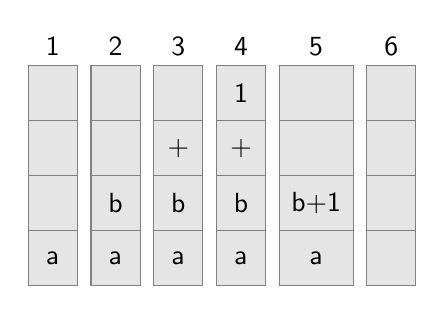
\begin{tikzpicture}[node distance=-0.5pt]
    \node [gray box=2] (10) {};
    \node [gray box=2, below=of 10] (11) {}; 
    \node [gray box=2, below=of 11] (12) {};
    \node [gray box=2, below=of 12] (13) {a};
    \node [gray box=2, right=of 10, xshift=5pt] (20) {};
    \node [gray box=2, below=of 20] (21) {}; 
    \node [gray box=2, below=of 21] (22) {b};
    \node [gray box=2, below=of 22] (23) {a};
    \node [gray box=2, right=of 20, xshift=5pt] (30) {};
    \node [gray box=2, below=of 30] (31) {+}; 
    \node [gray box=2, below=of 31] (32) {b};
    \node [gray box=2, below=of 32] (33) {a};
    \node [gray box=2, right=of 30, xshift=5pt] (40) {1};
    \node [gray box=2, below=of 40] (41) {+}; 
    \node [gray box=2, below=of 41] (42) {b};
    \node [gray box=2, below=of 42] (43) {a};
    \node [gray box=3, right=of 40, xshift=5pt] (50) {};
    \node [gray box=3, below=of 50] (51) {}; 
    \node [gray box=3, below=of 51] (52) {b+1};
    \node [gray box=3, below=of 52] (53) {a};
    \node [gray box=2, right=of 50, xshift=5pt] (60) {};
    \node [gray box=2, below=of 60] (61) {}; 
    \node [gray box=2, below=of 61] (62) {};
    \node [gray box=2, below=of 62] (63) {};
    \node [annotation, above] at (10.north) {1};
    \node [annotation, above] at (20.north) {2};
    \node [annotation, above] at (30.north) {3};
    \node [annotation, above] at (40.north) {4};
    \node [annotation, above] at (50.north) {5};
    \node [annotation, above] at (60.north) {6};
  \end{tikzpicture}
\end{multicols}
\vspace{-2.5em}

\section{In Class Quiz 2 - Slide 14}
Is the given scope stack correct for location D of the given code?  \textbf{Yes}
\vspace{-1em}
\begin{multicols}{2}
  \textb{
\vspace{-1em}
\begin{algorithmic}[1]
  \Begin
    \State declare H, A, L: integer; \textbfr{ $\leftarrow$ A}
    \Begin
      \Begin
        \State declare X, Y: Real; \textbfr{ $\leftarrow$ B}
      \End; \textbfr{ $\leftarrow$ C}
      \Begin
        \State declare A, C, M: char; \textbfr{ $\leftarrow$ D}
      \End;
    \End;
  \End;
\end{algorithmic}
  }
  \vfill\columnbreak
  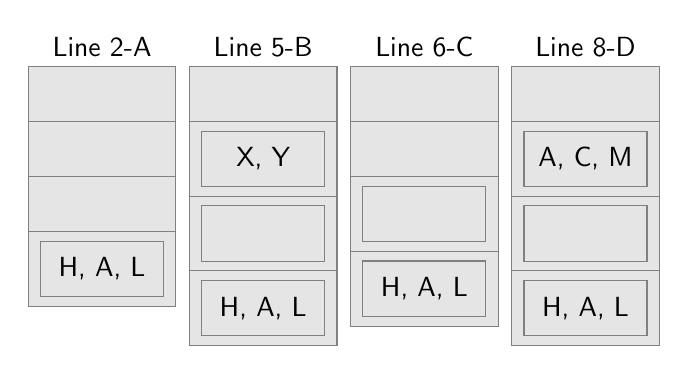
\begin{tikzpicture}[node distance=-0.5pt]
    \node [gray box=6] (10) {};
    \node [gray box=6, below=of 10] (11) {}; 
    \node [gray box=6, below=of 11] (12) {};
    \node [gray box=6, below=of 12] (13) {\tikz{\node[gray box=5] {H, A, L};}};
    \node [gray box=6, right=of 10, xshift=5pt] (20) {};
    \node [gray box=6, below=of 20] (21) {\tikz{\node[gray box=5] {X, Y};}}; 
    \node [gray box=6, below=of 21] (22) {\tikz{\node[gray box=5] {};}};
    \node [gray box=6, below=of 22] (23) {\tikz{\node[gray box=5] {H, A, L};}};
    \node [gray box=6, right=of 20, xshift=5pt] (30) {};
    \node [gray box=6, below=of 30] (31) {}; 
    \node [gray box=6, below=of 31] (32) {\tikz{\node[gray box=5] {};}};
    \node [gray box=6, below=of 32] (33) {\tikz{\node[gray box=5] {H, A, L};}};
    \node [gray box=6, right=of 30, xshift=5pt] (40) {};
    \node [gray box=6, below=of 40] (41) {\tikz{\node[gray box=5] {A, C, M};}}; 
    \node [gray box=6, below=of 41] (42) {\tikz{\node[gray box=5] {};}};
    \node [gray box=6, below=of 42] (43) {\tikz{\node[gray box=5] {H, A, L};}};
    \node [annotation, above] at (10.north) {Line 2-A};
    \node [annotation, above] at (20.north) {Line 5-B};
    \node [annotation, above] at (30.north) {Line 6-C};
    \node [annotation, above] at (40.north) {Line 8-D};
  \end{tikzpicture}
\end{multicols}
\vspace{-2em}


\section{In Class Quiz 3 - Slide 19}
Which sequence of actions are invoked for the string: \textbfb{INT a;} \\
var\_decl $\rightarrow$ var\_type id; \textr{\#decl\_id} \\
var\_type $\rightarrow$ INT \textr{\#int\_type} | FLOAT \textr{\#float\_type} \\
id $\rightarrow$ IDENTIFIER \textr{\#id} \\
Action sequence: \textbf{\#int\_type,\#id, \#decl\_id}
\vspace{-1em}
\begin{multicols}{2}
\begin{enumerate}
  \item int\_type() generate a record for "int"
  \item id() generates a record for "a"
  \item decl\_id() pop the two top most records \\
  and invokes ex $\rightarrow$ insert\_entry(int, a) \\
  if not in table add it, if already in table $\rightarrow$ error
\end{enumerate}
  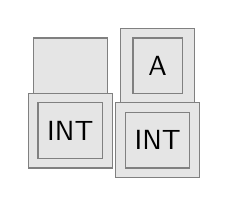
\begin{tikzpicture}[node distance=-0.5pt]
    \node [gray box=3] (10) {};
    \node [gray box=3, below=of 10] (11) {\tikz{\node[gray box=2] {INT};}};
    \node [gray box=3, right=of 10, xshift=5pt] (20) {\tikz{\node[gray box=2] {A};}};
    \node [gray box=3, below=of 20] (21) {\tikz{\node[gray box=2] {INT};}};
  \end{tikzpicture}
\end{multicols}


\section{Abstract Syntax Tree (AST) - In Class Quiz 6 - Slide 40}
\vspace{-1em}
\begin{multicols}{2}Draw the complete AST for: \textbfb{w := x + y * (z + 3)}. How many leaf nodes are included? \\
Post Order: \textbf{w, x, y, z, 3, +, *, +, :=} \\
Leaf nodes: \textbf{5} \\
    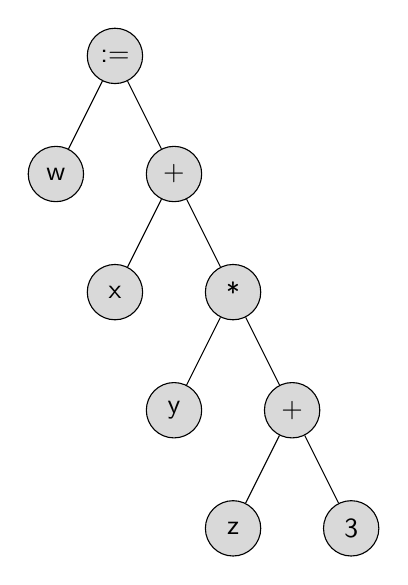
\begin{tikzpicture}
    \node[vertex]
    {:=}
        child {
            node[vertex] {w}
        } child {
            node[vertex] {+}
            child { node[vertex] {x} }
            child {
                node[vertex] {*}
                child { node[vertex] {y} }
                child {
                    node[vertex] {+}
                    child { node[vertex] {z} }
                    child { node[vertex] {3} }
                }
            }
        }
    ;
  \end{tikzpicture} \\
\end{multicols}

\vspace{-8em}
\section{Generating Three-Address Code (3AC) from AST}
L-value := R-value
\begin{description}
  \item [L-values]: addresses which can be stored to or loaded from
  \item [R-values]: data (often loaded from addresses)
  \item [C]: a constant
\end{description} \ \\
  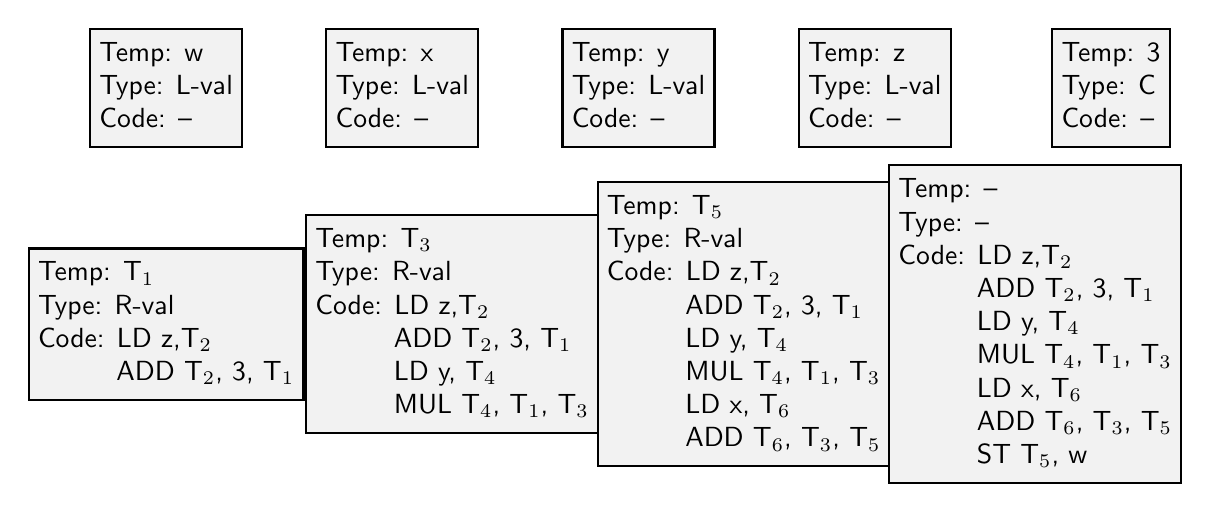
\begin{tikzpicture}
    \node[state, shape=rectangle] (0) {
    \makecell[l] {
    Temp: w \\
    Type: L-val \\
    Code: --
    }};
    \node[state, shape=rectangle, right of=0] (1) {
    \makecell[l] {
    Temp: x \\
    Type: L-val \\
    Code: --
    }};
    \node[state, shape=rectangle, right of=1] (2) {
    \makecell[l] {
    Temp: y \\
    Type: L-val \\
    Code: --
    }};
    \node[state, shape=rectangle, right of=2] (3) {
    \makecell[l] {
    Temp: z \\
    Type: L-val \\
    Code: --
    }};
    \node[state, shape=rectangle, right of=3] (4) {
    \makecell[l] {
    Temp: 3 \\
    Type: C \\
    Code: --
    }};
    \node[state, shape=rectangle, below of=0] (4) {
    \makecell[l] {
    Temp: T$_1$ \\
    Type: R-val \\
    Code: LD z,T$_2$ \\
    \hspace{2.5em} ADD T$_2$, 3, T$_1$
    }};
    \node[state, shape=rectangle, right of=4, xshift=18pt] (5) {
    \makecell[l] {
    Temp: T$_3$ \\
    Type: R-val \\
    Code: LD z,T$_2$ \\
    \hspace{2.5em} ADD T$_2$, 3, T$_1$ \\
    \hspace{2.5em} LD y, T$_4$ \\
    \hspace{2.5em} MUL T$_4$, T$_1$, T$_3$
    }};
    \node[state, shape=rectangle, right of=5, xshift=20pt] (6) {
    \makecell[l] {
    Temp: T$_5$ \\
    Type: R-val \\
    Code: LD z,T$_2$ \\
    \hspace{2.5em} ADD T$_2$, 3, T$_1$ \\
    \hspace{2.5em} LD y, T$_4$ \\
    \hspace{2.5em} MUL T$_4$, T$_1$, T$_3$ \\
    \hspace{2.5em} LD x, T$_6$ \\
    \hspace{2.5em} ADD T$_6$, T$_3$, T$_5$
    }};
    \node[state, shape=rectangle, right of=6, xshift=20pt] (7) {
    \makecell[l] {
    Temp: -- \\
    Type: -- \\
    Code: LD z,T$_2$ \\
    \hspace{2.5em} ADD T$_2$, 3, T$_1$ \\
    \hspace{2.5em} LD y, T$_4$ \\
    \hspace{2.5em} MUL T$_4$, T$_1$, T$_3$ \\
    \hspace{2.5em} LD x, T$_6$ \\
    \hspace{2.5em} ADD T$_6$, T$_3$, T$_5$ \\
    \hspace{2.5em} ST T$_5$, w
    }};
  \end{tikzpicture}


\section{In Class Quiz 7 - Slide 51}
\vspace{-1em}
\begin{multicols}{2}
Draw the AST for \textbfb{ x := z + 3}. What is the order of nodes visited when performing post-order traversal? \\
Post Order: \textbf{x, z, 3, +, :=} \\
  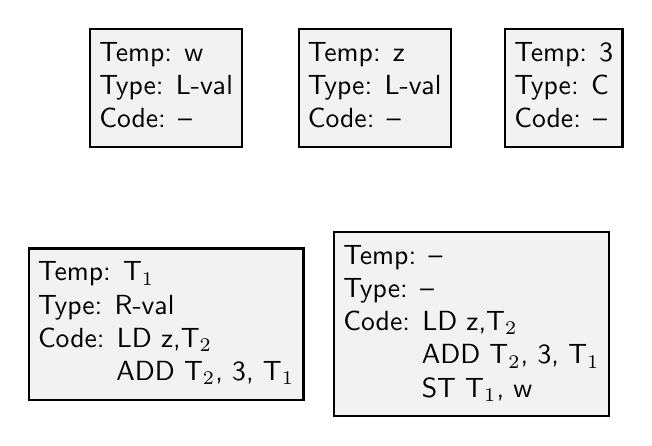
\begin{tikzpicture}
    \node[state, shape=rectangle] (0) {
    \makecell[l] {
    Temp: w \\
    Type: L-val \\
    Code: --
    }};
    \node[state, shape=rectangle, right of=0, xshift=-10pt] (1) {
    \makecell[l] {
    Temp: z \\
    Type: L-val \\
    Code: --
    }};
    \node[state, shape=rectangle, right of=1, xshift=-17pt] (2) {
    \makecell[l] {
    Temp: 3 \\
    Type: C \\
    Code: --
    }};
    \node[state, shape=rectangle, below of=0] (3) {
    \makecell[l] {
    Temp: T$_1$ \\
    Type: R-val \\
    Code: LD z,T$_2$ \\
    \hspace{2.5em} ADD T$_2$, 3, T$_1$
    }};
    \node[state, shape=rectangle, right of=3, xshift=25pt] (4) {
    \makecell[l] {
    Temp: -- \\
    Type: -- \\
    Code: LD z,T$_2$ \\
    \hspace{2.5em} ADD T$_2$, 3, T$_1$ \\
    \hspace{2.5em} ST T$_1$, w
    }};
  \end{tikzpicture}
\end{multicols}
\vspace{-12em}
\indent \hspace{10em}
  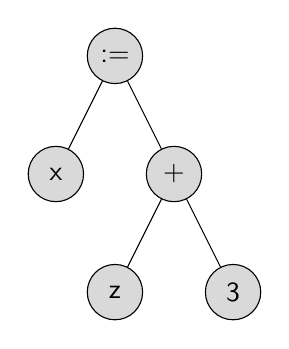
\begin{tikzpicture}
    \node[vertex]
    {:=}
        child {
            node[vertex] {x}
        } child {
            node[vertex] {+}
            child { node[vertex] {z} }
            child { node[vertex] {3} }
        }
    ;
  \end{tikzpicture}

\section{In Class Quiz 8 - Slide 52}
Draw the AST for \textbfb{x := z + 3}. Assume you perform post-order traversal
on this AST to generate code. How many lines of code are included in
the data object for the root node? \textbf{3} Lines of code


\chapter{Semantic Actions for Control Structures}
\section{Generate 3AC for If-elseif}
\vspace{-1em}
\begin{multicols}{2}
If-elseif statement: \\
\textr{if <bool\_expr\_1>} \\
\indent \textr{<stmt\_list\_1>} \\
\textb{else if <bool\_expr\_2>} \\
\indent \textb{<stmt\_list\_2>} \\
\textp{else} \\
\indent \textp{<stmt\_list\_3>} \\
\textg{Endif}


\subsection{In Class Quiz 1 - Slide 9}
\vspace{.5em}
Generate 3AC for the given if-elseif statement.
How many unconditional jumps and labels are included? \\
\textbf{2 jumps, 3 labels}
  \vfill\columnbreak
Generated assembly code: \\
\indent \textr{<code for bool\_expr\_1>} \\
\indent \textr{j<!op> ELSE\_1} \\
\indent \textr{<code for stmt\_list\_1>} \\
\indent \textr{jmp OUT\_1} \\
\textb{ELSE\_1:} \\
\indent \textb{<code for bool\_expr\_2>} \\
\indent \textb{j<!op> ELSE\_2} \\
\indent \textb{<code for stmt\_list\_2>} \\
\indent \textb{jmp OUT\_2} \\
\textp{ELSE\_2:} \\
\indent \textp{<code for stmt\_list\_3>} \\
\textg{OUT\_1:}
\end{multicols}


\section{Generate 3AC for While Loops}
\vspace{-1em}
\begin{multicols}{2}
while \textr{<bool\_expr>} \\
\indent \textb{<stmt\_list>} \\
endwhile;


\subsection{In Class Quiz 2 - Slide 14}
\vspace{1em}
In the previous While loop, what is the 3AC \\ 
for a \textit{break} statement? \textbf{jmp OUT}
  \vfill\columnbreak
LOOP: \\
\indent \textr{<bool\_expr>} \\
\indent j<!op> OUT \\
\indent \textb{<stmt\_list>} \\
\indent jmp LOOP \\
OUT:
\end{multicols}

\section{Generate 3AC for For Loops}
\vspace{-1em}
\begin{multicols}{2}
for (\textr{<init\_stmt>};\textb{<bool\_expr>};\textg{<incr\_stmt>}) \\
\indent \textp{<stmt\_list>} \\
end


\subsection{In Class Quiz 3 - Slide 19}
In the previous For loop, what is the 3AC \\
for a \textit{continue} statement?
\textbf{jmp INCR}
  \vfill\columnbreak
\indent \textr{<init\_stmt>} \\
LOOP: \\
\indent \textb{<bool\_expr>} \\
\indent j<!op> OUT \\
\indent \textp{<stmt\_list>} \\
INCR: \\
\indent \textg{<incr\_stmt>} \\
\indent jmp LOOP \\
OUT:
\end{multicols}

\section{Generate 3AC for Switch Statements}
\vspace{-1em}
\begin{multicols}{2}
switch (<expr>) \\
\indent case <const\_list>: <stmt\_list> \\
\indent case <const\_list>: <stmt\_list> \\
\indent ... \\
\indent default: <stmt\_list> \\
end
  \vfill\columnbreak
\indent <expr> \\
\indent <code for jump table> \\
LABEL0: \\
\indent <stmt\_list> \\
LABEL1: \\
\indent <stmt\_list> \\
\indent ... \\
DEFAULT: \\
\indent <stmt\_list> \\
OUT:
\end{multicols}


\setcounter{chapter}{6}
\chapter{Code Generation \& Local Optimization}
\section{Naïve approach}
\vspace{-1em}
\begin{multicols}{6}
 \ \\
\textr{MUL A,4,B} \\
\vfill\columnbreak
 \ \\
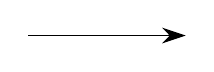
\begin{tikzpicture}
\draw [-{Stealth[length=3mm, width=2mm]}] (0,0) -- (2,0);
\end{tikzpicture}
\vfill\columnbreak
\textr{LD A,R1} \\
\textr{MOV 4,R2} \\
\textr{MUL R1,R2,R3} \\
\textr{ST R3,B}
\vfill\columnbreak
 \ \\
\textb{MUL A,4,B}
\vfill\columnbreak
 \ \\
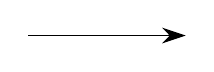
\begin{tikzpicture}
\draw [-{Stealth[length=3mm, width=2mm]}] (0,0) -- (2,0);
\end{tikzpicture}
\vfill\columnbreak
\textb{LD A,R1} \\
\textb{MUL R1,4,R3} \\
\textb{ST R3,B}
\end{multicols}
\vspace{-1em}
\textbf{Too many instructions. Could use a different instruction type.} \\


\vspace{-1.5em}
\subsection{Activity - Slide 5}
\vspace{-1em}
\begin{multicols}{6}
 \ \\
ADD A,B,C $\longrightarrow$
\vfill\columnbreak
LD A,R1 \\
LD B,R2 \\
ADD R1,R2,R3 \\
ST R3,C
\vfill\columnbreak
 \ \\
ADD C,A,E $\longrightarrow$
\vfill\columnbreak
LD C,R4 \\
LD A,R5 \\
ADD R4,R5,R6 \\
ST R6,E
\vfill\columnbreak
 \ \\
ADD A,B,D $\longrightarrow$
\vfill\columnbreak
LD A,R7 \\
LD B,R8 \\
ADD R7,R8,R9 \\
ST R9,D
\end{multicols}
\vspace{-1em}
\textbf{Reduce loads of A, B, C. Reduce compuation of A + B. Too may registers.} \\


\vspace{-1.5em}
\section{Peephole optimizations}
\vspace{-1em}
\begin{itemize}
\begin{multicols}{2}
  \item Constant folding \\
    \textr{ADD lit1, lit2, Rx} $\longrightarrow$  \textb{MOV lit1 + lit2, Rx} \\
    \textr{MOV lit1, Rx} $\longrightarrow$ \textb{MOV lit1 + lit2, Ry} \\
    \textr{ADD li2, Rx, Ry}
  \item Strength reduction \\
    \textr{MUL operand, 2, Rx} $\longrightarrow$ \textb{SHIFTL operand, 1, Rx} \\
    \textr{DIV operand, 4, Rx} $\longrightarrow$ \textb{SHIFTR operand, 2, Rx}
  \item Null sequences \\
    \textr{MUL operand, 1, Rx} $\longrightarrow$ \textb{MOV operand, Rx} \\
    \textr{ADD operand, 0, Rx} $\longrightarrow$ \textb{MOV operand, Rx}
\vfill\columnbreak
  \item Combine operations \\
    \textr{JEQ L1} \\
    \textr{JMP L2} $\longrightarrow$ \textb{JNE L2} \\
    \textr{L1: ...}
  \item Simplifying \\
    \textr{SUB 0,, operand Rx} $\longrightarrow$ \textb{NEG operand Rx}
  \item Special cases (taking advantage of ++/--) \\
    \textr{ADD 1, Rx, Rx} $\longrightarrow$ \textb{INC Rx} \\
    \textr{SUB Rx, 1, Rx} $\longrightarrow$ \textb{DEC Rx}
  \item Address mode operations \\
    \textr{MOV A R1} \\
    \textr{ADD 0(R1) R2 R3} $\longrightarrow$ \textb{ADD @A R2 R3}
\end{multicols}
\end{itemize}

\vspace{-3em}
\section{Common Subexpression Elimination (CSE)}
\vspace{-1em}
\begin{multicols}{4}
Three address code \\
+ A B T1  \\
+ T1 C T2 \\
+ A B T3  \\
+ T1 T2 C \\
+ T1 C T4 \\
+ T3 T2 D
\vfill\columnbreak
Generated code \\
ADD A B R1 \\
ADD R1 C R2 \\
MOV R1 R3 \\
ADD R1 R2 R5; ST R5 C \\
ADD R1 C R4 \\
ADD R3 R2 R6; ST R6 \\
(C in R5, no need for R6)
\vfill\columnbreak
Available Expressions \\
"A+B", T1 \\
\st{"T1+C", T2} (killed) \\

"T1+T2", C  (updates C) \\
"T1+C", T4 \\
"T3+T2", D \\
\vfill\columnbreak
CSE Missed \\
T1 = A + B \\
T2 = A + B + C \\
T3 = A + B \\
C  = 2A + 2B + C \\

D  = 2A + 2B + C \\
(D = C)
\end{multicols}

\subsection{In Class Quiz 1 - Slide 34}
\vspace{-1em}
\begin{multicols}{2}
Optimize the given code by performing CSE. \\
Assume it is the complete code. How many \\
computations in total can be eliminated? \textbf{1}
\vspace{-1em}
  \begin{multicols}{3}
    \begin{enumerate}
      \item b := a * a;
      \item c := a * a;
      \item d := b + c;
      \item e := b + b;
    \end{enumerate}
\vfill\columnbreak
 \ \\
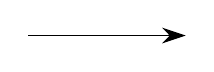
\begin{tikzpicture}
\draw [-{Stealth[length=3mm, width=2mm]}] (0,0) -- (2,0);
\end{tikzpicture}
\vfill\columnbreak
    \begin{enumerate}
      \item b := a * a;
      \item \textbf{c := b};
      \item d := b + c;
      \item e := b + b;
    \end{enumerate}
  \end{multicols}
\end{multicols}


\vspace{-2em}
\subsection{In Class Quiz 2 - Slide 35}
\vspace{-1em}
\begin{multicols}{2}
Optimize the given code by performing CSE. \\
Assume it is the complete code. How many \\
expressions are available after executing line 4? \textbf{3} \\
Live expressions: \textbf{a * a, b + c, b + b}
\vspace{-1em}
  \begin{multicols}{3}
    \begin{enumerate}
      \item b := a * a;
      \item c := a * a;
      \item d := b + c;
      \item e := b + b;
    \end{enumerate}
\vfill\columnbreak
 \ \\
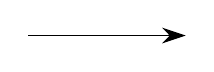
\begin{tikzpicture}
\draw [-{Stealth[length=3mm, width=2mm]}] (0,0) -- (2,0);
\end{tikzpicture}
\vfill\columnbreak
    \begin{enumerate}
      \item b := \textbf{a * a};
      \item c := b;
      \item d := \textbf{b + c};
      \item e := \textbf{b + b};
    \end{enumerate}
  \end{multicols}
\end{multicols}


\chapter{Register Allocation}
\section{Top Down Allocation - Slide 7}
\vspace{-1em}
\begin{multicols}{2}
  \begin{enumerate}
    \item A = 7
    \item B = A + 2
    \item C = A + B
    \item D = C + B
    \item B = C + B
    \item A = A + B
    \item E = C + D
    \item F = C + D
    \item G = A + B
    \item H = E + F
  \end{enumerate}
  A = 4	- Used the most \\
  B = 5	- Used the most \\
  C = 4	- Used the most \\
  D = 2 \\
  E = 1 \\
  F = 1 \\
  G = 0 \\
  $\leftarrow$ after this line C is no longer used\\
\end{multicols}
\vspace{-1em}
3 Registers $\rightarrow$ Use them to keep A, B, C. Need at least 1 more register, 2 more for register spilling \\
R1, R2, R3, R4 $\leftarrow$ could be used for register spilling \\
B, \hspace{.75em}A, \hspace{.5em}C



\section{Liveness}
\vspace{-1em}
\begin{multicols}{2}
\subsection{Example 1 - Slides 9-10}
\begin{tabular}{c|l|c|l|>{\bfseries}l}
  \textbf{No.} &  & \textbf{Defined} & \textbf{Used} & \textbf{Live} \\
  \hline
   1  & A = B + C   & A  & B, C  & \{A, B\}        \\
   2  & C = A + B   & C  & A, B  & \{A, B, C\}     \\
   3  & T1 = B + C  & T1 & B, C  & \{A, B, C, T1\} \\
   4  & T2 = T1 + C & T2 & T1, C & \{A, B, C, T2\} \\
   5  & D = T2      & D  & T2    & \{A, B, C, D\}  \\
   6  & E = A + B   & E  & A, B  & \{C, D, E\}     \\
   7  & B = E + D   & B  & E, D  & \{B, C, D\}     \\
   8  & A = C + D   & A  & C, D  & \{A, B\}        \\
   9  & T3 = A + B  & T3 & A, B  & \{T3\}          \\
  10  & WRITE(T3)   & -- & T3    & \{\}            \\
\end{tabular}
\vfill\columnbreak
\setlength{\leftskip}{3em}
\subsection{Example 2 - Slides 11-12}
\begin{tabular}{c|l|c|l|>{\bfseries}l}
  \textbf{No.} &  & \textbf{Defined} & \textbf{Used} & \textbf{Live} \\
  \hline
   1  & a := 0            & a  & a    & \{a, c\} \\
   2  & b := a + 1        & b  & b    & \{b, c\} \\
   3  & c := c + b        & c  & c, b & \{b, c\} \\
   4  & a := b * 2        & a  & b    & \{a, c\} \\
   5  & if a < 10 goto L1 & -- & a    & \{c\}    \\
   6  & return c          & -- & c    & \{\}     \\
\end{tabular}
\end{multicols}


\vspace{-1em}
\subsection{In Class Quiz 1 - Slide 14}
\vspace{-1em}
\begin{multicols}{2}
Perform Liveness analysis on the given code. There should
be 8 live sets (one each after executing the 8 lines of code). \\
How many live sets contain exactly 3 variables? \textbf{3}
\vfill\columnbreak
\begin{tabular}{c|l|c|l|>{\bfseries}l}
  \textbf{No.} &  & \textbf{Defined} & \textbf{Used} & \textbf{Live} \\
  \hline
   1  & v := 0            & v  & --      & \{v\}       \\
   2  & z := v + 1        & z  & v       & \{v, z\}    \\
   3  & x := z * v        & x  & z, v    & \{x, z\}    \\
   4  & y := x * 2        & y  & x       & \{x, y, z\} \\
   5  & w := x + z * y    & w  & x, z, y & \{w, y, z\} \\
   6  & u := z + 2        & u  & z       & \{u, w, y\} \\
   7  & v := u + w + y    & v  & u, w, y & \{u, v\}    \\
   8  & return v * u      & -- & u, v    & \{\}        \\
\end{tabular}
\end{multicols}


\section{Global Register Allocation (with graph coloring)}
3 - colorable graph - 3 registers needed \\
Edges are live, each pair of variables live together will be connected in graph. \\
Colors represent the number of available registers \\


\renewcommand\thechapter{E2}
\chapter{Final Exam - Practice Questions}
\section{Q1}
Draw the abstract syntax tree along with the data object of the root node for
the following piece of code: \\ \textbfr{a := b + c * d + e} \\
\scalebox{.8}{
  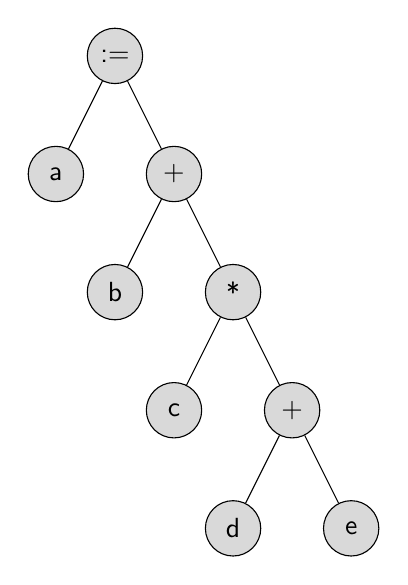
\begin{tikzpicture}
    \node[vertex]
    {:=}
        child {
            node[vertex] {a}
        } child {
            node[vertex] {+}
            child { node[vertex] {b} }
            child {
                node[vertex] {*}
                child { node[vertex] {c} }
                child {
                    node[vertex] {+}
                    child { node[vertex] {d} }
                    child { node[vertex] {e} }
                }
            }
        }
    ;
  \end{tikzpicture} \\
}
\scalebox{.9}{
  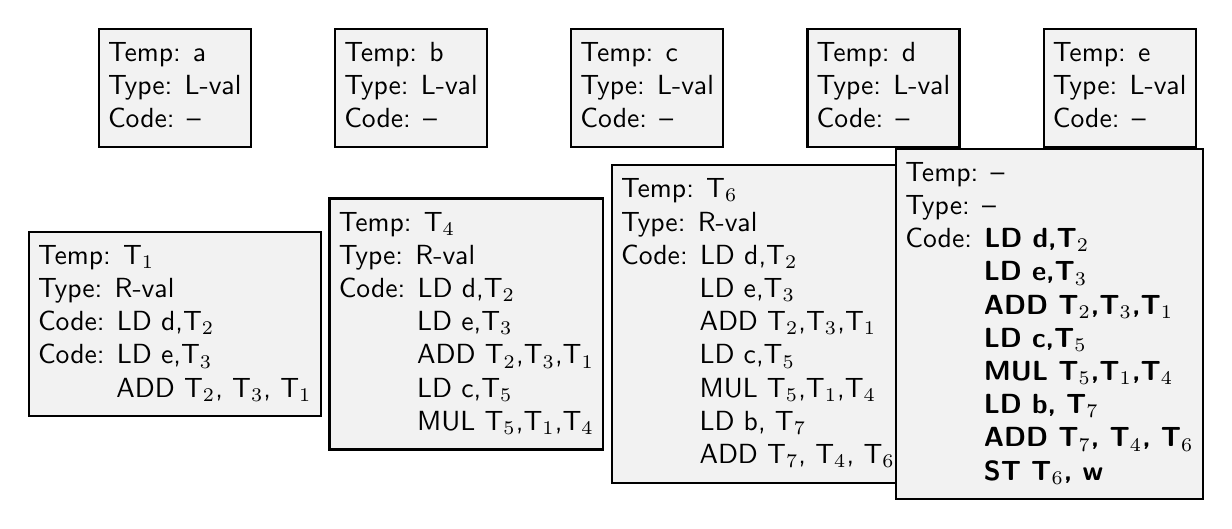
\begin{tikzpicture}
    \node[state, shape=rectangle] (0) {
    \makecell[l] {
    Temp: a \\
    Type: L-val \\
    Code: --
    }};
    \node[state, shape=rectangle, right of=0] (1) {
    \makecell[l] {
    Temp: b \\
    Type: L-val \\
    Code: --
    }};
    \node[state, shape=rectangle, right of=1] (2) {
    \makecell[l] {
    Temp: c \\
    Type: L-val \\
    Code: --
    }};
    \node[state, shape=rectangle, right of=2] (3) {
    \makecell[l] {
    Temp: d \\
    Type: L-val \\
    Code: --
    }};
    \node[state, shape=rectangle, right of=3] (4) {
    \makecell[l] {
    Temp: e \\
    Type: L-val \\
    Code: --
    }};
    \node[state, shape=rectangle, below of=0] (4) {
    \makecell[l] {
    Temp: T$_1$ \\
    Type: R-val \\
    Code: LD d,T$_2$ \\
    Code: LD e,T$_3$ \\
    \hspace{2.5em} ADD T$_2$, T$_3$, T$_1$
    }};
    \node[state, shape=rectangle, right of=4, xshift=20pt] (5) {
    \makecell[l] {
    Temp: T$_4$ \\
    Type: R-val \\
    Code: LD d,T$_2$ \\
    \hspace{2.5em} LD e,T$_3$ \\
    \hspace{2.5em} ADD T$_2$,T$_3$,T$_1$ \\
    \hspace{2.5em} LD c,T$_5$ \\
    \hspace{2.5em} MUL T$_5$,T$_1$,T$_4$
    }};
    \node[state, shape=rectangle, right of=5, xshift=20pt] (6) {
    \makecell[l] {
    Temp: T$_6$ \\
    Type: R-val \\
    Code: LD d,T$_2$ \\
    \hspace{2.5em} LD e,T$_3$ \\
    \hspace{2.5em} ADD T$_2$,T$_3$,T$_1$ \\
    \hspace{2.5em} LD c,T$_5$ \\
    \hspace{2.5em} MUL T$_5$,T$_1$,T$_4$ \\
    \hspace{2.5em} LD b, T$_7$ \\
    \hspace{2.5em} ADD T$_7$, T$_4$, T$_6$
    }};
    \node[state, shape=rectangle, right of=6, xshift=20pt] (7) {
    \makecell[l] {
    Temp: -- \\
    Type: -- \\
    Code: \textbf{LD d,T$_2$} \\
    \hspace{2.5em} \textbf{LD e,T$_3$} \\
    \hspace{2.5em} \textbf{ADD T$_2$,T$_3$,T$_1$} \\
    \hspace{2.5em} \textbf{LD c,T$_5$} \\
    \hspace{2.5em} \textbf{MUL T$_5$,T$_1$,T$_4$} \\
    \hspace{2.5em} \textbf{LD b, T$_7$} \\
    \hspace{2.5em} \textbf{ADD T$_7$, T$_4$, T$_6$} \\
    \hspace{2.5em} \textbf{ST T$_6$, w}
    }};
  \end{tikzpicture}
}


\vspace{-2em}
\section{Q2}
Consider the following piece of code:
\begin{center}
  \begin{tabular}{|c|l|>{\bfseries}l|>{\bfseries}l|>{\bfseries}l|}
    \hline
  	& Code & Available$_1$ & Code$_2$ & Available$_3$ \\
    \hline
    1: & A = B + C & B + C & A = B + C & --    \\
    2: & B = B + C & --    & B = A     & --    \\
    3: & Q = A + C & A + C & Q = A + C & A + C \\
    4: & A = A + C & --    & A = Q     & --    \\
    5: & P = B + C & B + C & B = B + C & B + C \\
    \hline
  \end{tabular} \ \\
\end{center}
\begin{enumerate}
  \item Assume there is no aliasing between variables. For each statement, list which expressions are "available" \textit{after} the statement executes.
  \item What does the code look like after performing CSE? Leave the code in IR form.
When eliminating a redundant expression, replace it with the variable that holds
the previous result of computing the expression.
  \item How would your response to part 2 change if A and B were aliased? \\
  \textbf{Statement 2 would not longer be redundant \\ (because statement 1 would immediately kill "B+C")}
\end{enumerate}

\section{Q3}
Consider the following code (assume this is the full program):
\vspace{-1em}
\begin{multicols}{2}
\begin{enumerate}
  \item Show which variables and temporaries are live after each instruction (assume
no aliasing)
  \item Consider Instruction 7 in the code.\\
   What variables would be live after instruction 7 if A may be aliased to B and C. \\
   \textbf{Instruction 8 uses A \& B \& may use C \\
   (because A may be aliased to C) \\
   \{A,B\} $\Rightarrow$ \{A,B,C\}}
\end{enumerate}
  \begin{tabular}{|c|l|>{\bfseries}l|>{\bfseries}l|>{\bfseries}l|}
    \hline
  	& Code & Def & Use & Live \\
    \hline
     1: & A = 7       & A  & --   & {A,C}    \\
     2: & B = 8       & B  & --   & {A,B,C}  \\
     3: & T1 = A + B  & T1 & A,B  & {A,B,C,T1} \\
     4: & T2 = T1 + C & T2 & T1,C & {A,B,T2} \\
     5: & C = A + B   & C  & A,B  & {B,C,T2} \\
     6: & T3 = T2 + C & T3 & T2,C & {B,C,T3} \\
     7: & A = C + T3  & A  & C,T3 & {A,B}    \\
     8: & T4 = A + B  & T4 & A,B  & {A,T4}   \\
     9: & B = A + T4  & B  & A,T4 & {B}      \\
    10: & WRITE(B)    & -- & B    & {}       \\
    \hline
  \end{tabular}
\end{multicols}


\section{Q4}
\vspace{-1em}
\begin{multicols}{2}
Assume you have a machine with 2 ALUs (ALU0 and ALU1) and one LD/ST unit.
Your instruction set consists of 5 instructions: ADD, MUL, LOAD and STORE. An
ADD instruction can be performed on either ALU, and takes one cycle. A MUL
instruction can be performed on ALU0 or ALU1, and takes two cycles. A LOAD
takes up either of the ALUs for one cycle, then the LD/ST unit for two cycles. A
STORE takes up either of the ALUs for one cycle, then the LD/ST unit for one cycle.
All of the functional units are fully pipelined. Draw the reservation tables for the
instructions.
  \vfill\columnbreak
  \begin{tabular}{|c|>{\bfseries}c|>{\bfseries}c|>{\bfseries}l|>{\bfseries}l|}
    \hline
  	& ALU0   & ALU1 & LD/DT \\
    \hline
    ADD(1)   & X &   &  \\
    \hline
    ADD(2)   &   & X &  \\
    \hline
    MUL(1)   & X &   &  \\
             &   &   &  \\
    \hline
    MUL(2)   &   &   &  \\
             &   &   &  \\
    \hline
    LD(1)    & X &   &   \\
             &   &   & X \\
             &   &   &  \\
    \hline
    STORE(1) & X &   &   \\
             &   &   & X \\
    \hline
    STORE(2) &   & X &   \\
             &   &   & X \\
    \hline
  \end{tabular}
\end{multicols}

\section{Q5}
Draw the data dependence graph for the following piece of code. Don't forget to label the dependence edges with their latency
\vspace{-1em}
\begin{multicols}{2}
\begin{enumerate}
  \item R1 = LOAD(A)
  \item R2 = LOAD(B)
  \item R3 = LOAD(C)
  \item R4 = R2 + R1
  \item R5 = R4 * R1
  \item R6 = R1 + R2
  \item R7 = R4 + R6
  \item R8 = R5 * R6
  \item R9 = R8 + R7
  \item R10 = R3 * R9
  \item D = STORE(R10)
\end{enumerate}
6 can be 7 or 8, max(7,8) = 8 \\
  \begin{tabular}{|c|>{\bfseries}c|>{\bfseries}c|>{\bfseries}l|>{\bfseries}l|}
    \hline
  	Cycle & ALU0   & ALU1 & LD/DT \\
    \hline
     0 &  1 &   &    \\
    \hline
     1 &  2 &   & 1  \\
    \hline
     2 &  3 &   & 2  \\
    \hline
     3 &    &   & 3  \\
    \hline
     4 &  4 & 6 &    \\
    \hline
     5 &  5 & 7 &    \\
    \hline
     6 &    &   &    \\
    \hline
     7 &  8 &   &    \\
    \hline
     8 &    &   &    \\
    \hline
     9 &  9 &   &    \\
    \hline
    10 & 10 &   &    \\
    \hline
    11 &    &   &    \\
    \hline
    12 & 11 &   &    \\
    \hline
    13 &    &   & 11 \\
    \hline
  \end{tabular}
  \vfill\columnbreak
  \setlength{\leftskip}{-2em}
  \begin{tikzpicture}[->, >=stealth', node distance=2cm]
    \node[state] (1) {1};
    \node[state, above of=4, right of=4] (2) {2};
    \node[state, below of=2] (4) {4};
    \node[state, right of=2] (3) {3};
    \node[state, below of=4, left of=4] (5) {5};
    \node[state, below of=4, right of=4] (6) {6};
    \node[state, below of=4] (7) {7};
    \node[state, below of=7, left of=7] (8) {8};
    \node[state, below of=6, right of=7] (9) {9};
    \node[state, right of=9] (10) {10};
    \node[state, right of=10] (11) {11};
    \draw[very thick]
      (1) edge[left, below, bend right=20] node{3} (4)
      (1) edge[left, left] node{3} (5)
      (1) edge[left, left, bend left=50] node{3} (6)
      (2) edge[left, right] node{3} (4)
      (2) edge[left, right, bend left=20] node{3} (6)
      (3) edge[left, right] node{3} (10)
      (4) edge[left, above] node{1} (5)
      (4) edge[left, left] node{1} (7)
      (5) edge[left, left] node{2} (8)
      (6) edge[left, above] node{1} (7)
      (6) edge[left, right] node{1} (8)
      (7) edge[left, above] node{1} (9)
      (8) edge[left, above] node{2} (9)
      (9) edge[left, above] node{1} (10)
      (10) edge[left, above] node{2} (11);
    \node [annotation, left] at (1.west) {\tikz{\node[gray box=1] {13};}};
    \node [annotation, above, left] at (2.west) {\tikz{\node[gray box=1] {13};}};
    \node [annotation, right] at (3.east) {\tikz{\node[gray box=1] {7};}};
    \node [annotation, right] at (4.east) {\tikz{\node[gray box=1] {10};}};
    \node [annotation, left] at (5.west) {\tikz{\node[gray box=1] {9};}};
    \node [annotation, right] at (6.east) {\tikz{\node[gray box=1] {8};}};
    \node [annotation, left] at (7.west) {\tikz{\node[gray box=1] {6};}};
    \node [annotation, below] at (8.south) {\tikz{\node[gray box=1] {7};}};
    \node [annotation, below] at (9.south) {\tikz{\node[gray box=1] {5};}};
    \node [annotation, below] at (10.south) {\tikz{\node[gray box=1] {4};}};
    \node [annotation, below] at (11.south) {\tikz{\node[gray box=1] {2};}};
  \end{tikzpicture} \ \\
  
  \textbf{Order 1, 2, 3, 4, 6, 5, 7, 8, 9, 10, 11} \\

  \textbf{14 Cycles to complete}
\end{multicols}

\end{document}
